\section{Rappels géométriques.}

\begin{prop} 
  L'aire d'un rectangle dont les côtés sont de longueurs $a$ et $b$ est $ab$. 
\end{prop}

\begin{prop}
  L'aire d'un trapèze de hauteur $h$ et de côtés de longueurs $a$ et $b$ est $h\times \dfrac{a+b}{2}$.
\end{prop}



\section{Méthodes géométriques.}

L'objectif est d'approcher le réel $  \int_a^b f$ où $a$ et $b$ sont deux réels (on supposera $a<b$) et où $f$ est une fonction réelle définie sur le segment $[a,b]$.

Les méthodes les plus simples reposent toutes sur le même principe. 
\begin{itemize}
  \item On subdivise le segment $[a,b]$ en $n$ segments : $[x_0,x_1]$, ..., $[x_{n-1},x_n]$ avec, pour tout $0 \leq k \leq n$, $x_k = a + k\dfrac{b-a}{n}$.
  \item Sur chaque segment $[x_{k-1},x_{k}]$, on approche $\displaystyle\int_{x_{k-1}}^{x_{k}} f$ par l'intégrale d'une fonction, que l'on espère proche de $f$. 
  \item On renvoie la somme de ces $n$ intégrales comme approximation de $\displaystyle\int_a^b f$.
\end{itemize}

L'objectif est dans chaque cas d'obtenir une approximation précise de l'intégrale à calculer, avec une complexité modérée. Notamment, nous utiliserons la définition suivante. 

\begin{defi}[Erreur d'approximation]
  Soit $A_n$ une approximation de $\displaystyle\int_a^b f$ obtenue à partir de $n$ segments. L'\emph{erreur d'approximation} de $\displaystyle\int_a^b f$ par $A_n$ est $    \abs{\displaystyle\int_a^b f - A_n}$.
\end{defi}


\subsection{Méthode(s) des rectangles.}

Cette méthode a été (ou sera bientôt) étudiée en détails dans le cours de mathématiques. 

Pour chaque subdivision, on choisit un $t_k\in[x_{k-1},x_{k}]$ et l'on approche la fonction $f$ sur $[x_{k-1},x_{k}]$ par la valeur $f(t_k)$, on approche donc $\displaystyle\int_{x_{k-1}}^{x_{k}} f$ par $\dfrac{b-a}{n} f(t_k)$ et l'approximation de  $\displaystyle\int_a^b f$ obtenue est donc $ \dfrac{b-a}{n} \sum_{k=1}^n f(t_k)$.
Il y a donc autant de méthodes des rectangles que de manières de choisir ces nombres $t_1,\dots,t_n$. On n'en étudiera que deux. 



\subsubsection{Méthode des rectangles à gauche.}

Pour chaque $1 \leq k \leq n$, on choisit la borne gauche de $[x_{k-1},x_{k}]$, soit $x_{k-1}$.

L'approximation de  $\displaystyle\int_a^b f$ calculée est donc $  R_n = \dfrac{b-a}{n} \sum_{k=1}^n f\p{a+(k-1)\dfrac{b-a}{n}}$.

On code très simplement cette méthode, comme suit. 

\begin{pyverbatim}
def Rg(f,a,b,N):
    """Approximation de l'intégrale de a à b de f 
    Méthode des rectangles à gauche, N rectangles"""
    S = 0
    h = (b-a)/N
    for k in range(N) : 
        S = S + f(a + k*h)
    return S*h
\end{pyverbatim}

\subsubsection{Méthode des rectangles à droite.}

Pour chaque $1 \leq k \leq n$, on choisit la borne droite de $[x_{k-1},x_{k}]$, soit $x_k$.

L'approximation de  $\displaystyle\int_a^b f$ calculée est donc $
  R_n' = \dfrac{b-a}{n} \sum_{k=1}^n f\p{a+k\dfrac{b-a}{n}}$.


On code très simplement cette méthode, comme suit. 

\begin{pyverbatim}
def Rd(f,a,b,N):
    """Approximation de l'intégrale de a à b de f 
    Méthode des rectangles à droite, N rectangles"""
    S = 0
    h = (b-a)/N
    for k in range(1,N+1) : 
        S = S + f(a + k*h)
    return S*h
\end{pyverbatim}

\subsubsection{Propriétés communes.}

On démontre dans le cours de mathématiques les propriétés suivantes. 

\begin{prop}
  Soit $a,b \in \R$ avec $a<b$, soit $f : [a,b] \to \R$. 
  \begin{enumerate}
    \item Si $f$ est continue, alors toute approximation de $\displaystyle\int_a^b f$ par une méthode des rectangles converge vers $\displaystyle\int_a^b f$. 
    \item Si $f$ est lipschitzienne, alors toute méthode des rectangles a une erreur d'approximation en $O\p{\dfrac{1}{n}}$. 
  \end{enumerate}
\end{prop}

Les propriétés suivantes sont immédiates. 

\begin{prop}
  Soit $a,b \in \R$ avec $a<b$, soit $f : [a,b] \to \R$. 
  \begin{enumerate}
    \item Si $f$ est constante, alors toute méthode des rectangles est exacte. 
    \item On a $R_n - R_n' = (f(a)-f(b))\dfrac{b-a}{n}$. Si $f(a) \neq f(b)$, l'erreur d'approximation d'une des deux méthodes des rectangles (à gauche ou à droite) est exactement de l'ordre de $\dfrac{1}{n}$. 
  \end{enumerate}
\end{prop}

\begin{rem}
  En plus du calcul de la subdivision, le calcul d'une approximation par la méthode des rectangles avec $n$ rectangles demande donc $n$ appels à la fonction $f$ et $n$ addition (plus une multiplication de flottants).
\end{rem}

\subsection{Méthode des trapèzes.}

Pour chaque subdivision, on approche la fonction $f$ sur $[x_{k-1},x_{k}]$ par la corde à la courbe de $f$ sur le segment $[x_{k-1},x_{k}]$, on approche donc $\displaystyle\int_{x_{k-1}}^{x_{k}} f$ par $\dfrac{b-a}{2n}\p{f(x_{k-1}) + f(x_k)}$ et l'approximation de  $\displaystyle\int_a^b f$ obtenue est donc 
\begin{align*}
  T_n &= \dfrac{b-a}{2n} \sum_{k=1}^n \p{f\p{a+(k-1)\dfrac{b-a}{n}} + f\p{a+k\dfrac{b-a}{n}}} \\
      &= \dfrac{S_n + S_n'}{2} \\
      &= \dfrac{b-a}{n}\p{ \dfrac{f(a)}{2} + \sum_{k=1}^{n-1}  f\p{a+k\dfrac{b-a}{n}} + \dfrac{f(b)}{2}}.
\end{align*}

\begin{rem}
  Dans la dernière écriture, on a pris soin d'effectuer le moins d'opérations possible. 
\end{rem}

On code très simplement cette méthode, comme suit. 

\begin{pyverbatim}
def T(f,a,b,N):
    """Approximation de l'intégrale de a à b de f 
    Méthode des trapèzes, N trapèzes"""
    S = 0.5*(f(a) + f(b))
    h = (b-a)/N
    for k in range(1,N) : 
        S = S + f(a + k*h)
    return S*h
\end{pyverbatim}

On a les propriétés suivantes. 

\begin{prop}
  Soit $a,b \in \R$ avec $a<b$, soit $f : [a,b] \to \R$. 
  \begin{enumerate}
    \item Si $f$ est continue, alors l'approximation de $\displaystyle\int_a^b f$ par la méthode des trapèzes converge vers $\displaystyle\int_a^b f$. 
    \item Si $f$ est $\mathscr{C}^2$, alors la méthode des trapèzes a une erreur d'approximation en $O\p{\dfrac{1}{n^2}}$. 
    \item Si $f$ est affine, alors la méthode des trapèzes est exacte. 
  \end{enumerate}
\end{prop}

\begin{rem}
  En plus du calcul de la subdivision, le calcul d'une approximation par la méthode des trapèzes avec $n$ trapèzes demande donc $n+1$ appels à la fonction $f$ et $n+1$ addition (plus quelques opérations sur les flottants).
\end{rem}

\subsection{Supplément : méthode de Simpson.}

Pour chaque subdivision, on approche la fonction $f$ sur $[x_{k-1},x_{k}]$ par la fonction polynomiale de degré 2 coïncidant avec $f$ en $x_{k-1}$, $\dfrac{x_{k-1} + x_k}{2}$ et en $x_k$, on approche donc $\displaystyle\int_{x_{k-1}}^{x_{k}} f$ par $\dfrac{b-a}{6n}\p{f(x_{k-1}) + 4 f\p{\dfrac{x_{k-1} + x_k}{2}}+ f(x_k)}$ et l'approximation de  $\displaystyle\int_a^b f$ obtenue est donc 
%\begin{align*}
%  S_n &= \dfrac{b-a}{6n} \sum_{k=1}^n \p{f\p{a+(k-1)\dfrac{b-a}{n}}+ 4f\p{a+\p{k-\dfrac{1}{2}}\dfrac{b-a}{n}} + f\p{a+k\dfrac{b-a}{n}}} \\
%      &= \dfrac{b-a}{6n} \p{ f(a) + 2 \sum_{k=1}^{n-1}  f\p{a+k\dfrac{b-a}{n}} + 4 \sum_{k=1}^{n}  \p{k-\dfrac{1}{2}} f\p{a+k\dfrac{b-a}{n}}+  f(b)}.
%\end{align*}

\begin{align*}
  S_n &= \dfrac{b-a}{6n} \sum_{k=1}^n \p{f\p{a+(k-1)\dfrac{b-a}{n}}+ 4f\p{a+\p{k-\dfrac{1}{2}}\dfrac{b-a}{n}} + f\p{a+k\dfrac{b-a}{n}}} \\
      &= \dfrac{b-a}{6n} \p{ f(a) + 2 \sum_{k=1}^{n-1}  f\p{a+k\dfrac{b-a}{n}} + 4 \sum_{k=1}^{n}  \p{a+\p{k-\dfrac{1}{2}}\dfrac{b-a}{n}}+  f(b)}.
\end{align*}

\begin{rem}
  Dans la dernière écriture, on a pris soin d'effectuer le moins d'opérations possible. 
\end{rem}

On a les propriétés suivantes. 

\begin{prop}
  Soit $a,b \in \R$ avec $a<b$, soit $f : [a,b] \to \R$. 
  \begin{enumerate}
    \item Si $f$ est continue, alors l'approximation de $\displaystyle\int_a^b f$ par la méthode de Simpson converge vers $\displaystyle\int_a^b f$. 
    \item Si $f$ est $\mathscr{C}^4$, alors la méthode de Simpson a une erreur d'approximation en $O\p{\dfrac{1}{n^4}}$. 
    \item Si $f$ est polynomiale de degré au plus deux, alors la méthode de Simpson est exacte. 
  \end{enumerate}
\end{prop}


% [On met le code ou ils le font en TP ???]

\subsection{Représentation graphique de ces différentes méthodes.}
On représente l'approximation de la courbe d'une fonction sur un segment, par ces quatres méthodes (voir figure~\ref{fig.integrales}).

\begin{figure}[!h]
  \begin{center}
    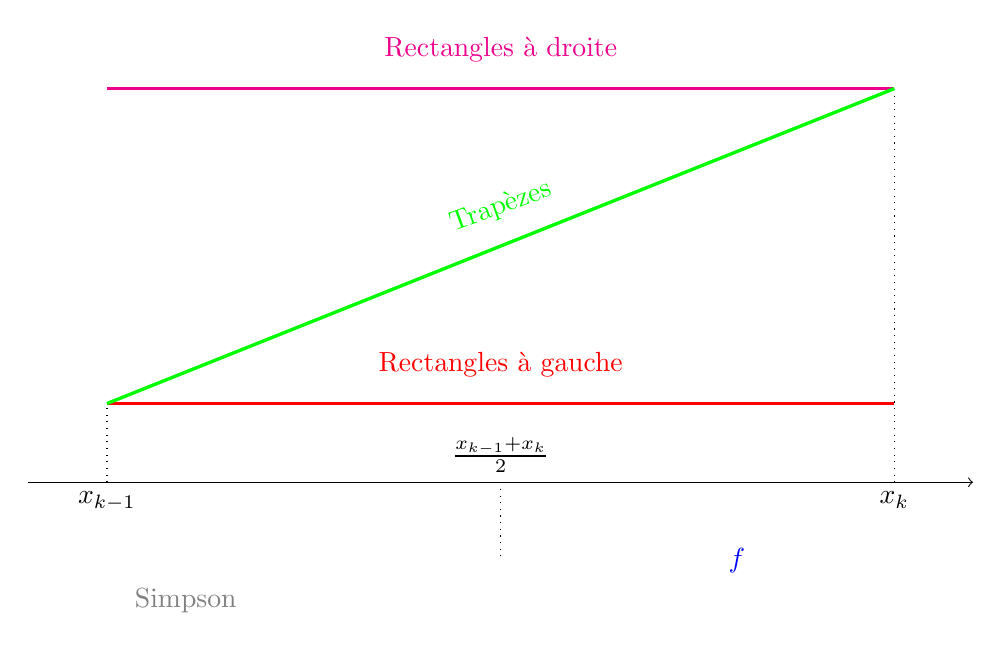
\begin{tikzpicture}
      \draw[->] (-1,0) -- (11,0) ;
      \draw[dotted] (0,0) node[anchor = north] {$x_{k-1}$} -- (0,1) ;
      \draw[dotted] (10,0) node[anchor = north] {$x_{k}$} -- (10,5) ;
      \draw[dotted] (5,0) node[anchor = south] {$\frac{x_{k-1}+x_{k}}{2}$} -- (5,-1) ;
      \draw[blue,very thick] plot[smooth] file {integrales_f.dat};
      \draw[red,very thick] (0,1) -- (10,1) ;
      \draw[magenta,very thick] (0,5) -- (10,5) ;
      \draw[green,very thick] (0,1) -- (10,5) ;
      \draw[gray,very thick] plot[smooth] file {integrales_simpson.dat};
      \draw[blue,very thick] (8,-1) node{$f$};
      \draw[red,very thick] (5,1.5) node{Rectangles à gauche};
      \draw[magenta,very thick] (5,5.5) node{Rectangles à droite};
      \draw[gray,very thick] (1,-1.5) node{Simpson};
      \draw[green,very thick] (5,3.5) node[rotate=20]{Trapèzes};
    \end{tikzpicture}
    \caption{Approximations sur $[x_{k-1},x_{k}]$ de la fonction $f$ utilisées.}
    \label{fig.integrales}
  \end{center}
\end{figure}

\section{Intégration numérique fournie par \python.}

La bibliothèque \texttt{scipy.integrate} contient la fonction \texttt{quad}, qui met en \oe{}uvre une méthode numérique de calcul approché d'intégrales. 
Elle utilise la bibliothèque Fortran QUADPACK. 
Les méthodes numériques utilisées sont bien plus complexes que celles présentées ici, mais reposent sur la même idée : approcher l'intégrale de la fonction par une combinaison linéaire d'évaluations de cette fonction, les points d'évaluation et les poids étant judicieusement choisis. 

On remarquera que la fonction \texttt{quad} peut prendre en argument une précision et donne un résultat dont l'erreur d'approximation est inférieure à cette précision ! 


